\documentclass[11pt,aspectratio=169,dvipsnames]{beamer}
\graphicspath{{figs/}}
\usetheme{default}
\usepackage{DasBeamerPaket}
\usepackage{animate}
\usepackage{lastpage}
\usepackage{appendixnumberbeamer}
\usepackage{braket}
\usepackage{booktabs}
\usepackage{tabularx}
\usepackage{tikz}
\usepackage{eso-pic}
\setbeamercolor{section in toc}{fg=NavyBlue}
\setbeamercolor{frametitle}{fg=NavyBlue}
\captionsetup[figure]{labelfont=bf}
\captionsetup[table]{labelfont=bf}
\newcommand{\theauthor}{Jakob Krause}
\newcommand{\theshortauthor}{\textsc{J. Krause} for CBELSA/TAPS}
\newcommand{\authormail}{krause@hiskp.uni-bonn.de}
\newcommand{\authorgit}{krausejm}
\newcommand{\thetitle}{Recent Polarization Observable Results in  $\eta$- and $\eta'$-photoproduction off the proton}
\newcommand{\theshorttitle}{$\Sigma$ in $\eta$- and $\eta'$ photoproduction}
\newcommand{\thecolor}{black!70!blue}
\newcommand{\thecolorr}{black!60!blue}
\newcommand{\thecolorrr}{black!50!blue}
\newcommand{\thesubtitle}{Master thesis for the CBELSA/TAPS collaboration}
\newcommand{\thedate}{30th March 2022}
\makeatletter
\patchcmd{\beamer@calculateheadfoot}{\advance\footheight by 4pt}{\advance\footheight by 20pt}{}{}
\makeatother

\begin{document}
	\definecolor{myWhite}{rgb}{1,1,1}
	
	
	\setbeamercolor{coloredboxstuff}{fg=myWhite,bg=\thecolor}
	\setbeamercolor{coloredboxstuff1}{fg=myWhite,bg=\thecolorr}
	\setbeamercolor{coloredboxstuff2}{fg=myWhite,bg=\thecolorrr}	
	
	
	\makeatother
	\setbeamertemplate{footline}
	{
		\leavevmode%
		\hbox{%
			\begin{beamercolorbox}[wd=.34\paperwidth,ht=2.25ex,dp=1ex,center]{coloredboxstuff}%
				{\theshortauthor}
			\end{beamercolorbox}%
			\begin{beamercolorbox}[wd=.34\paperwidth,ht=2.25ex,dp=1ex,center]{coloredboxstuff1}%
				{\theshorttitle}
			\end{beamercolorbox}%
			\begin{beamercolorbox}[wd=.34\paperwidth,ht=2.25ex,dp=1ex,center]{coloredboxstuff}%
				\insertframenumber{} / \inserttotalframenumber\hspace*{1ex}
		\end{beamercolorbox}}%
	}
	\makeatletter
	
	
	\setbeamercovered{transparent}
	\setbeamertemplate{navigation symbols}{}
	\setbeamertemplate{frametitle}[default][left,leftskip=0.5cm]
	\setbeamertemplate{itemize item}{\color{black}$\blacktriangleright$}
	\setbeamertemplate{section in toc}[sections numbered]
	\setbeamercolor{section in toc}{fg=\thecolor}
	\setbeamercolor{frametitle}{fg=\thecolor}
	\captionsetup{font=scriptsize,labelfont=scriptsize}
	
	
	
	
	\begin{frame}[plain,noframenumbering]
		
		\centering
\begin{minipage}{.49\linewidth}
			\begin{tcolorbox}[colback=red!5,colframe=red!50!black,title=Before]
				Point estimate: $\Sigma_{\chi^2}\pm\Delta(\Sigma_{\chi^2})$
			\end{tcolorbox}
\end{minipage}
\begin{minipage}{.49\linewidth}
		\begin{tcolorbox}[colback=green!5,colframe=green!50!black,title=Now]
				marginal posteriors: $p(\Sigma|y)$
	\end{tcolorbox}
\end{minipage}
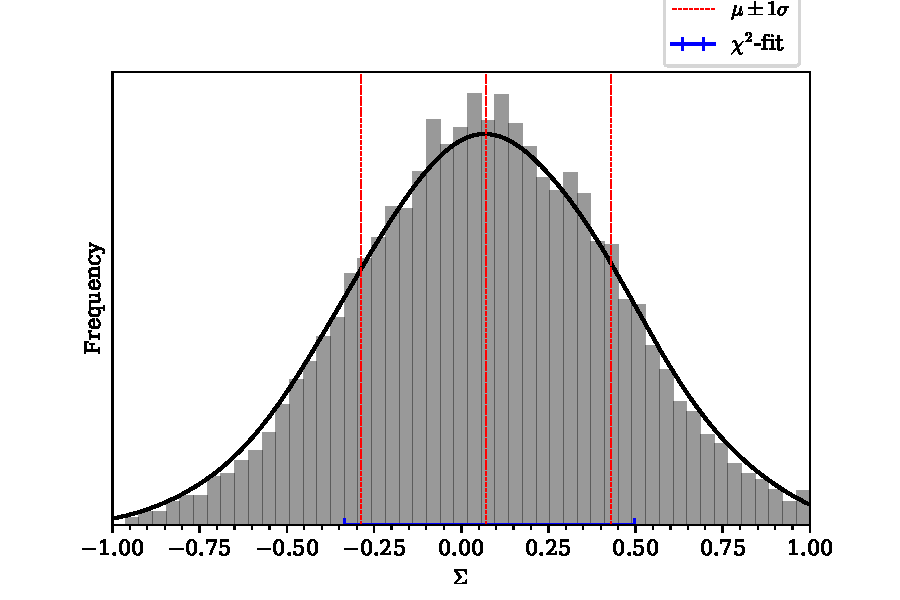
\includegraphics[width=.7\linewidth]{figs/posterior_1_params.pdf}
	\end{frame}
\end{document}